%-----------------------------------------------------------------------------
%
%               Template for sigplanconf LaTeX Class
%
% Name:         sigplanconf-template.tex
%
% Purpose:      A template for sigplanconf.cls, which is a LaTeX 2e class
%               file for SIGPLAN conference proceedings.
%
% Guide:        Refer to "Author's Guide to the ACM SIGPLAN Class,"
%               sigplanconf-guide.pdf
%
% Author:       Paul C. Anagnostopoulos
%               Windfall Software
%               978 371-2316
%               paul@windfall.com
%
% Created:      15 February 2005
%
%-----------------------------------------------------------------------------


\documentclass[10pt,reprint]{socc14}

\usepackage{amsmath}
\usepackage{mathptmx}
\usepackage{graphicx}
\usepackage{listings}
%\usepackage{cite}

\frenchspacing

\begin{document}
	
\special{papersize=8.5in,11in}
\setlength{\pdfpageheight}{\paperheight}
\setlength{\pdfpagewidth}{\paperwidth}

\conferenceinfo{Submission to SoCC '15}{August, 2015,  Kohala Coast, Hawaii, USA} 
\copyrightyear{2015} 
\copyrightdata{978-1-nnnn-nnnn-n/yy/mm} 
\doi{nnnnnnn.nnnnnnn}

% Uncomment one of the following two, if you are not going for the 
% traditional copyright transfer agreement.

%\exclusivelicense                % ACM gets exclusive license to publish, 
                                  % you retain copyright

%\permissiontopublish             % ACM gets nonexclusive license to publish
                                  % (paid open-access papers, 
                                  % short abstracts)

%\titlebanner{banner above paper title}        % These are ignored unless
%\preprintfooter{short description of paper}   % 'preprint' option specified.

\title{JSpeed.io: A Javascript Powered Distributed System For High Performance Computing}
%\subtitle{...}

\authorinfo{Victor Santos, Servio Palacios, Ananth Grama}
           {Department of Computer Science, Purdue University}
           {\{vsantosu,spalacio,ayg\}@purdue.edu}

\maketitle

\begin{abstract}
As the era of big data becomes mainstream, the need to process large datasets and intensive calculations in a batch and streaming fashion becomes a necessity. We present a new distributed system that offers trivial setup, simple still powerful programming model, and high level of abstraction without sacrificing performance, maintainability, and scalability. We cover how our system compares to similar implementations, its benefits and drawbacks, and our vision of potential applications. We expose how emerging technologies such as Node.js helped us to implementation sandboxing techniques in private, and crowd sourced execution points with high levels of abstraction. Our system has its specific programming model, which involves the implementation of distributed algorithms as finite state machines that switch states asynchronously at each internal or external event. This event-driven automaton programming model makes it possible to create high performance/non-blocking distributed algorithms without the need of any concurrent primitive such as locks, semaphores, and mutexes, and therefore simplifying the implementation and maintainability of the algorithms. We discuss how our system is structured to support multi-tenancy by using JavaScript’s higher order functions, closures and callbacks. The system implements cutting edge technologies such as WebSockets and WebRTC to create point to point communication between execution points with low latency and response time. We demonstrate almost linear scaling with the number of execution points (sandboxes) by executing several CPU and I/O bound algorithms such prime numbers calculations and MapReduce. Finally, we discuss different aspects including but not limited to: fault tolerance, security, and how unsolved problems such as the halting problem becomes a challenge at the moment of implementing a crowd sourced distributed system capable of in-browser execution\cite{Amazon}.
\end{abstract}

\category{CR-number}{subcategory}{third-level}

% general terms are not compulsory anymore, 
% you may leave them out
\terms
Distributed, Performance

\keywords
Event-Driven, Javascript, Cloud Computing, Crowdsourcing

\section{Introduction}

In present times, there have been a bursting grow big data related terms.  From real time analytics~\cite{Chen2012}, to data mining for business, complex datasets classification, and other buzz topics that involves a common element: large scale data processing. Since Google published the MapReduce paper in 2008~\cite{Dean2008}, researchers and industry have created different kinds of applications~\cite{Chu2007,Ekanayake2008,Papadimitriou2008}, on top of this framework to solve problems that are not necessarily suited for the MapReduce. In order to accomplish these solutions, the framework needs to be modified, or find a workaround for dependencies, group communication, or simply an alternative to what MapReduce does not support. All this is done with the sole purpose of getting massive processing speedup in this distributed system at the moment of analyzing gigabytes or petabytes of data. Although there are robust and well known frameworks [14] that can accomplish this, scientists and industry are inclined to use MapReduce based system such as Hadoop~\cite{Hadoop} to solve distributed and big data problems. Any person with experience in both MPI and Hadoop MapReduce know the difficulty difference at the moment of implementing an algorithm in both platforms. While plain message passing can be extremely flexible, algorithms can become complex and error prone due to synchronization, race conditions, and all standard concurrency primitives. On the other hand, the MapReduce framework takes those drawbacks away by providing a clean and straightforward API that abstract all communication and synchronization details from the user. The main problem with this simplicity and abstraction is that it loses flexibility and adapting several types of algorithms to this framework can be troublesome. In this study, we propose a new distributed system/framework that offers trivial setup, simple still powerful programming model, and high level of abstraction without sacrificing performance, maintainability, and scalability. We are aiming to provide a system with the ability of solving large scale problems in high-end and commodity hardware(even mobile devices) with flexibility, simplicity, yet high  performance. The system takes advantage of emerging technologies[3] and the maturity of some others~\cite{Tilkov2010} in order to accomplish our target functionality. This paper contains all the details of our early implementation and concepts and is organized as follows: 

Section 2 briefly discuss related research and systems. In this section we discuss how existing systems such as SETI@Home~\cite{Korpela2001a}, CrowdCL~\cite{MacWilliam2013}, River Trail~\cite{Herhut2013a}, Hadoop \cite{Hadoop}, and MPI~\cite{GroppWilliamandLuskEwingandSkjellum1999} bring together the inspiration and the fundamentals of our system. We present the advantages and disadvantages of each system and how our proposed solution tackles those disadvantages to fit and keep complying with each system original purpose.

Section 3 explains all the implementation details and concepts of our system. This includes:structure, workflow, execution points sandboxing~\cite{Agten2012,Mckeown2008}, fault tolerance, communication, data structures, and the flexible boundaries of the system. This section contains technical details about the implementation engineering and the asynchronous nature of Node.js, and consequently  how this  influence great part of the system design. We also explain how the previous research~\cite{Haller2009} contributes to implementing the event-driven concurrency in our system. The system's programming model will be explained in detail in this section. The event-driven finite state machine programming model is one of the most critical concepts of the system. We contrast this model with existing parallel/distributed programming patterns such as message passing~\cite{GroppWilliamandLuskEwingandSkjellum1999}, and how different algorithms are accomplished with traditional concurrency primitives(locks, mutex, semaphores) and not blocking asynchronous mechanisms(promises, callbacks, signals, and events). Finally, we present the advantages in terms of performance of the JavaScript runtime~\cite{Tilkov2010}, and how emerging technologies~\cite{Herhut2013a,Yee2009} to reach nearly native execution performance. We also explain how to handle algorithms that are CPU and IO bound in both, Node.js and in-browser environment.

Section 4 presents several experiments that show the performance or our system  under different scenarios. From simple number crunching algorithms with no file system requirements, to a MapReduce implementation over Gigabytes of data with heavy I/O operations. We demonstrate how the system behaves in different scenarios, the communication cost, how faults affects the execution, and how to balance sandboxes with different capabilities (from cellphones, to high end servers).

Section 5 explains many important challenges and future work of our contributions. This section discusses the current challenges and what is ahead of the road in the next version of our system. Topics for this section are but not limited to: structural changes and programming model enhancements, fault tolerance or a real time system~\cite{Kopetz1989a}, decentralization and point to point communication~\cite{Vogt2013}, code optimization and existing applications porting~\cite{Zakai2011},  and the security of the execution points(sandboxes). Finally we briefly discuss the halting problem [10] in our system and the possible solutions~\cite{Alur1994}.

In section 6 we present our conclusions and insights.


\section{Design and Implementation}

Before we go into the further details of our system design and implementation, it’s imperative to enumerate several important facts.

Our system does not aim to replace existing solutions but to provide an alternate way to fulfill heavy distributed tasks using a different perspective and approach.
The system is based on emerging technologies, some of these are still in development~\cite{Vogt2013} and experimental~\cite{Herhut2013a,MacWilliam2013}. Many details in this section are not final and are subject to change as technologies are standardized and improved.
As mentioned in the previous section, our system aims to take advantage of crowdsourced computation, commodity hardware, and private dedicated machines for solely distributed processing purposes.
We have an experimental prototype of the system working, but not all features are fully implemented yet. Moreover, as this paper is being written, a full restructuration and refactoring of the codebase is taking place to implement all details mentioned ahead.

With the previous facts presented, let’s proceed to explore our system in the following eight sections.


\subsection{Technologies}
Our system heavily relies on relatively recent technologies. All functionalities run on top of any modern ECMAScript engine such as Google’s V8 engine,  Mozilla’s SpiderMonkey, Apple’s Nitro, and Microsoft Chakra. Our system is divided into two kind runtimes: 
Native: The native runtime uses Node.js V8 engine and has extended capabilities such as disk I/O and full OS interaction capabilities like any other modern language.
Browser: Any modern browser following the javaScript standard can become an execution point in our system. However, this runtime is strictly limited by the browser’s security policies such as no disk I/O, no direct OS interaction, and limited memory consumption.

javaScript was designed to be a simple scripting language for the web and not designed for performance, but we that is no longer true. javaScript has been the center of countless innovations and new technologies that supports real-time communication (WebSockets). Even the game industry is moving toward browser-based graphics processing (WebGL). In addition, there is a big ongoing effort to make javaScript a high-performance language similar to Java and even C++ [4, 6, 20]. Yet another reason for choosing javaScript as our main language is that tech giants such as Google and Mozilla have created runtimes with remarkable performance and scalability~\cite{Tilkov2010}.

Several important principles of our system are ruled by javaScript’s asynchronous nature. This is, perhaps, the most remarkable difference between our system and existing ones. Let's list the implications this nature on our system:

It does not rely on explicit multithreading to support concurrency at sandbox level, but in subworker processes that run on separated contexts.
It relies on a totally asynchronous I/O eventing model.
Its event-driven nature offer developers a more efficient and scalable alternative to application’s activity switching~\cite{Tilkov2010}.
Promises easier to implement distributed algorithms, maintainability and execution efficiency over those with explicit multi-threaded implementation~\cite{Tilkov2010}. 

\subsection{Programming Model}
One of our goals is to reduce the difficulty of plain multithreading programming and its common problems(deadlocks, shared resources collision, and race conditions). With the help of anonymous functions and closures, we maintain the context of all jobs isolated and ready to use at each asynchronous event. In this way, we prevent the use of global data and difficult to maintain data structures. Since the system is totally non-blocking, all I/O is handled asynchronously, therefore, no socket communication, disk IO, or messages from other nodes in the cluster blocks the execution or waste CPU cycles.

\subsubsection{The Asynchronous Finite State Machine}
The fact that javaScript does not support synchronization primitives, forces us to find an alternative to synchronizing and order algorithm’s execution flow in the top of its asynchronous nature. This is where we introduce our higher order functions assisted programming model, where all transitions in the algorithm are visualized as an asynchronous finite state machine. In this paper, we will be using the terms event and state interchangeably.

\begin{figure}[h]	
	\centering
	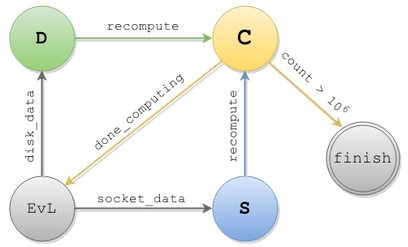
\includegraphics[scale=0.55]{AsynchronousAutomaton}
	\caption{Asynchronous automaton representation of a five state algorithm}
	\label{fig:AsynchronousAutomaton}
\end{figure}

Rather than implement threaded procedures with synchronization primitives, distributed algorithms in our system  must be represented as a finite state machine of events. In order to illustrate this idea, figure~\ref{fig:AsynchronousAutomaton} presents a simple distributed algorithm which consists of five states: 

Let state an example with figure~\ref{fig:AsynchronousAutomaton} structure. Given a large dataset containing a sequence of integer numbers, implement an algorithm that reads a section of the dataset from disk and compute the frequency of each integer in the entire dataset. We know that if the dataset contains terabytes of data, we would need to distributively execute this algorithm and receive data from other computing points in our system. In this case, we abstract our problem in states, where state D will asynchronously read from disk, S will receive the pair of <integer, frequency> list from a network socket, and C will compute/recompute these frequencies with the disk and network data, and finally finish the execution if a certain condition is met. In this previous example, we can notice that our algorithm executes according to events and transitions depending on those events. Moreover, we observe that all the I/O(i.e. disk and socket) is done asynchronously, meanwhile, other states can be executed concurrently. Continuing our previous example, if  we go from state EvL to D(data from disk), and at the same time we receive a socket\_data event, the internal event loop will take care of executing the queue of events and finally switch state to C where our computation will take place.

Now that we have seen the concept of how our system is meant to execute algorithms, we can make the following observations.
We code routines thinking of asynchronous events that will switch the states of our algorithm at any point in time.
The runtime itself leverage the synchronization of I/O operations, i.e. we don’t need to protect stored data structures from concurrent collisions.
Not suspension or blocking of states exist in this system. Instead, each event keeps it’s own context and when done, the event loop keeps idle or executes the next event.
We will encounter situations where we need to manage dependencies in our distributed computation, but we don’t have concurrency primitives such as semaphores and locks. We would need to differ asynchronous events if some dependency is not met. In order to do this, we use a combination of constructs (promises, signals, and emitters) which allow us to differ, signal, and emit asynchronous events at will. We briefly discuss how to handle dependencies and ordering of events in section 3.2.2.

%Figure 2
\begin{figure}	
	\centering
	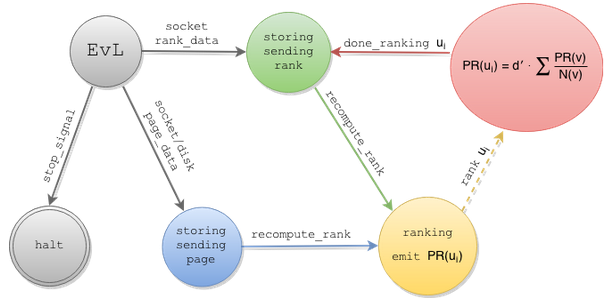
\includegraphics[scale=0.55]{AutomatonPageRank}
	\caption{Asynchronous automaton representation of the PageRank.}
	\label{fig:AutomatonPageRank}
\end{figure}


Figure~\ref{fig:AutomatonPageRank} shows a slightly more complex scenario. This time we present the asynchronous automaton representation of the Pagerank algorithm. 

\begin{equation}
	PR(u) =(1-d) + d\sum \frac{PR(v)}{N(v)}
\end{equation}

With the left side of the sum constant replaced by d’ for presentation simplicity:

\begin{equation}
  d' =(1-d) + d
\end{equation}

Analogous to the previous example, this automata has the default EvL state, and a termination state called halt, which indicates that this algorithm will halt on signal and not after a certain condition. It’s correct to infer that this is a streaming algorithm that will keep computing the received/read page ranks periodically. When a new page is read from disk, or it’s communicated via the network socket, the corresponding rank of that page is computed and stored asynchronously. Finally, the computed rank(if corresponds to this execution point) will be broadcasted to other execution points(Sandboxes) asynchronously.

\subsubsection{Handling state dependencies and ordering}
Dabek et. al. states that events are better means of managing I/O concurrency than threads since almost always have latent data races and deadlocks that make them less robust~\cite{Dabek2002}. In addition, they explicitly state that event-driven programs need only to allocate required memory for the event’s context, and not the whole thread stack, this way, dramatically reducing memory usage. The problem with the event-driven model is that lacks of synchronization primitives to logically state dependencies over asynchronous eventualities. This can be addressed by passing messages between events and used shared structures to differ events and reorder. This way synchronization becomes slightly clearer and reduces the number of global variables in compared to thread-based programs~\cite{Haller2009}.

Let’s go back to our figure~\ref{fig:AsynchronousAutomaton} example and suppose that we have a data dependency between state C(compute) and state D(read from disk). If state S(read from socket) is triggered several times before event D happens, the transition from state S to C can’t happen because the data dependency constraint is not met. In this case, we need to implement a different mechanism. 

%Figure 3
\begin{figure}[h]	
	\centering
	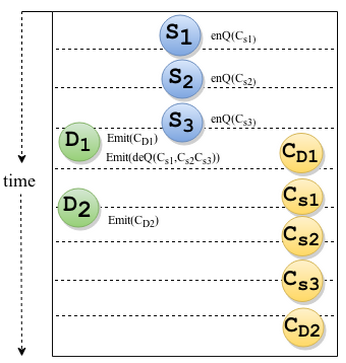
\includegraphics[scale=0.6]{StateDependency}
	\caption{State dependency scenario}
	\label{fig:StateDependency}
\end{figure}


Figure~\ref{fig:StateDependency} shows the previously exposed scenario where state S can’t move to the next state C if at least one event D happens first.  We can defer events S using asynchronous event emitter libraries~\cite{Caolan} and emit those events when event D happens. After this, our execution continues without problems. In figure~\ref{fig:StateDependency} we see that S happens three times before D, each time the event is put in a queue to later be rescheduled by event D. We have other mechanisms such as promises, callbacks and signals that can be combined to fulfill all kind of dependency and control flow scenarios.

%Architecture 

\subsection{Architecture}
Our system is composed of long-running daemons installed with just one command via the Node Package Manager~\cite{NPM}. Figure~\ref{fig:architectureDiagram} shows the peer-to-peer architecture of the system which is comprised of four main components. Each one of the components can be described as follows:
Clients: A client(group 2 in figure~\ref{fig:architectureDiagram})  is the starting point of all executions in the system. This is where we specify our distributed algorithm, the specific Sandboxes to be executed, the data sources, and the different settings of the execution. Each deployment is a job and we can have an arbitrary number of jobs executing at the same time.
Sandboxes: Each Sandbox(group 4 in figure~\ref{fig:architectureDiagram}) is a multi-tenant execution point where all deployed jobs run concurrently. Each time a client deploys a job, all target Sandboxes execute the asynchronous automaton code concurrently. In the next section, we will discuss in detail how the sandbox accomplishes each task.
Datasources: The Datasources(group 1 in figure~\ref{fig:architectureDiagram}) are any remote source that feeds the Job’s Sandboxes. This can be a streaming source, a remote filesystem, or a cloud storage service such as Amazon’s Cloud Drive~\cite{Amazon}.
Servers: Each server(group 1 in figure~\ref{fig:architectureDiagram})  has a register of each Sandbox, Client, and Datasources. The servers monitor every connection to the Sandboxes, clients and Datasources in real-time and notify every relevant change to the corresponding node, i.e. disconnection of a sandbox to an ongoing job’s client. The Server component is inspired by software-defined networking (SDN) Controllers~\cite{Mckeown2008}.


% FIGURE 4 Architecture Huge image
\begin{figure*}
	\centering
	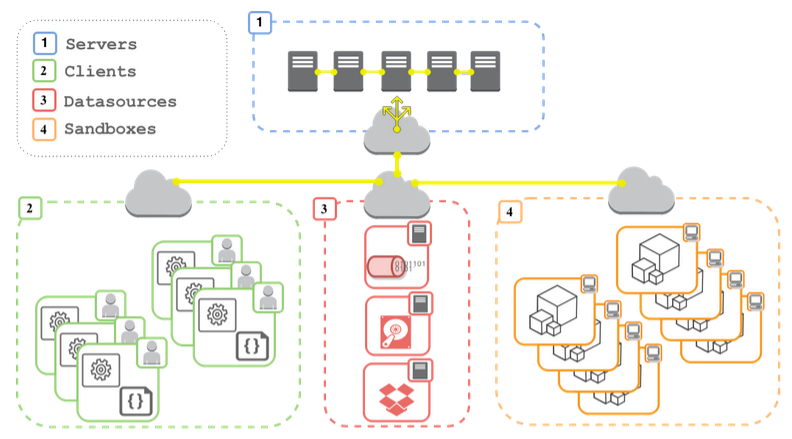
\includegraphics[scale=0.6]{architectureDiagram}
	\caption{Architecture of JSpeed.io which is comprised of four main components: Servers, Clients, Datasources, and Sandboxes.}
	\label{fig:architectureDiagram}
\end{figure*}


The system heavily relies on WebSockets. We are currently using the Socket.io \cite{Socket.} library for the real-time communication from which we leverage convenient features such as heartbeats, connection state, and event-driven communication. The Servers are continuously listening for connections from Clients, Sandboxes, and Datasources. Each time a new Sandbox connection comes in, the servers register the new node and broadcast its presence to Clients. At each disconnection, the Servers also broadcast the disconnection to Clients, in addition to fault tolerance messages if the Sandbox was executing a job.

\subsection{The Sandbox execution point}

The sandbox is perhaps the most complex component of our system. In its simplest form, the sandbox is a software of contention for executing third party javaScript routines in a distributed fashion. When a Sandbox is executed it follows following tasks:
Benchmark the performance of the environment(Node.js or Browser) in order to provide weighting metrics to the clients. These metrics will be used to fairly distribute job's loads among the group of selected Sandboxes at deployment time.
Spawn child process pool for jobs execution. Depending on the number of cores of the host, the Sandbox will spawn a subprocess pool where jobs will run. This is necessary since javaScript is single threaded, and each subprocess container will be handle isolated Job execution. Figure~\ref{fig:sandboxDiagram} shows how the sandbox contains two containers executing asynchronous automatons in an isolated manner.
Setup Job's queue structures/registers and inbound/outbound communication(Socket.io events).
Notify the Servers and send metrics(benchmark, NAT presence, IP, link speed, runtime capabilities, etc).
Wait in the event loop for events (Connection/Disconnection, Jobs). Socket.io takes care of the connection heartbeats for us.

This may look like a straightforward model. In fact, the Node.js version of the Sandbox is simple, efficient and with full capabilities of its environment. We simply spawn the subprocess pool and restrict functionality and resource consumption in those containers. The problem comes when the Sandbox executes in the browser. Since one of the targets of our system is crowdsourcing and easy setup(not need to install the Node.js Sandbox), is imperative to provide a secure and efficient runtime.

% Sandbox Diagram

\begin{figure}[h]	
	\centering
	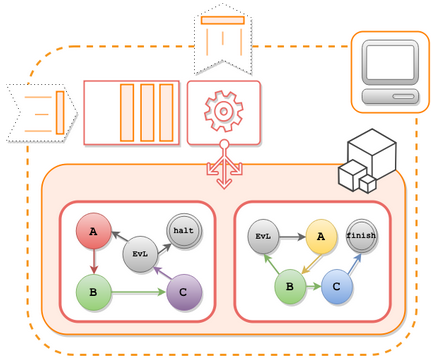
\includegraphics[scale=0.7]{sandboxDiagram}
	\caption{Architecture of the JSpeed.io’s sandbox.}
	\label{fig:sandboxDiagram}
\end{figure}

% Figure 4: Architecture of the JSpeed.io’s sandbox.

Without the proper security and regulations, the system could become the perfect DoS weapon, a free and accessible system with those capabilities could result in disaster. For ensuring complete isolation of deployed Jobs, we recur to the following sandboxing techniques:

HTML5 Web Workers: Web workers are deployed as a background process in the browser and are contained to just use Plain javaScript and XMLHttpRequest, no DOM objects are allowed. The problem with the web workers is that we are executing third party scripts(async automatons) as part of the distributed jobs. With access to do in-domain and different origin requests, we can fall into the mistake of allowing our system to become a DoS attack weapon. Static code analysis can be done to prevent this kind of situations, but the inclusion of libraries can make this process really difficult, even more in a scripting language like javaScript.
JSand~\cite{Agten2012}: JSand is a sandboxing framework implemented in javaScript that does not require browser modifications. In addition, JSand accesses all resources through the sandbox and enforces server-side policies without rewriting scripts or server-side filtering. Some sandboxing approaches require intrusive browser modifications, others do not support client-side script inclusion which effectively changes the architectural model of client-side script inclusion to server-side. Some approaches do not provide complete mediation between different scripts on the same page, or to all resources exposed in the browser.

Sandboxing techniques can protect the host machines of becoming a DoS and any access to DOM and Window objects. Still, there are other issues which we should be concerned. One of these problems is malicious deployed code that can deplete the host machine resources and even crash it. In section 3.8 we discuss a possible approach to this kind of problem.


\subsection{Fault Tolerance}
Our system is based on states of change and signals from external sources(peer Sandboxes), therefore, its ruled by the spontaneous initiatives of activities, which results in difficult to handle faults~\cite{Kopetz1989a}. According to Kopetz et. al. in this type of system we assume that components (Sandboxes, Clients, and Datasources) posses self-checking properties and fail silently. Moreover, they operate as intended, or do not produce any results. Since we have transient components, we would need redundant/synchronized self-checking nodes that as long as one of those components can operate, our required service can be maintained. Our system prototype implements a reschedule-if-fails policy. If we deploy a job with 20 Sandboxes, and 4 of them disconnect or fail, the payload of those 4 Sandboxes are rescheduled and gradually deployed when the first 4 of the 16 currently running finish their task. This without doubt degrades performance and currently only works with algorithms with not group communication requirements. Clearly inefficient, this approach at least guarantees the job’s completion as long as there is one Sandbox available. Fault tolerance will be a major area in the next development stage of the system.


\subsection{Limitations}
Our system has several limitations that are mainly due to the security and its client-server nature of web technologies. In the following subsections, we briefly discuss the two of this limitation.


\subsubsection{Browser Execution}
Currently, we can use two execution points: Any browser’s ECMAScript runtime, where users go to a web page and automatically setup all the execution environment and a Node.js application that currently runs on top of the V8 engine with full I/O and OS interaction capabilities. The browser runtime is limited to CPU-bound processes since it does not allow access to the file system because of security reasons. For this reason, we create the Datasource component which allows deployed jobs to fetch binary data from remote services, file systems, and streaming APIs. In addition to the previous limitation, we have the problem of not knowing the exact hardware capabilities of the machines. Some browsers support some host’s hardware information such as the number of CPU cores and bit architecture, but this certainly is not enough to precisely measure the power of the processing sandbox. At the setup of each Sandbox, we do a pessimistic approximation of the sandbox’s processing power by running a number crunching benchmark and calculating execution time.


\subsubsection{The Halting Problem}
One drawback we are facing in our system is the halting problem~\cite{Turing1937a}. It’s true that this is an unsolved problem that is present in any Turing Machine based computer. The problem is more noticeable in a system like ours where one of the targets is crowdsourcing. Every distributed execution is critical to the overall progress of the  algorithm, the question is if one particular sandbox will perpetually execute in an infinite loop or its gradually progressing towards the solution. A possible approach to this problem is the timed automata~\cite{Alur1994}. If we are running our sandbox in a Node.js environment, we then have the ability to monitor our job process and decide when to terminate if too much memory or CPU cycles are consumed. On the other hand, if we are in a browser, things get much more complicated since we don't have access to low-level OS information such as available memory and process execution. One possible solution is to extend our event-driven finite state machine model to a timed automata. We can extend our automata with real-valued variables in order to logically clock the execution. By using this technique, we can restrict the execution and behavior of our job and force it to switch into a termination state by following a certain policy.

\section{Experiments}

In order to present empirical evidence of JSpeed.io’s effectiveness, we designed two different experiments. First, we implemented the MapReduce algorithm and ran this job 16 times upon a 2GB CSV file. Each time, we incremented the number of native(Node.js) Sandboxes in order to obtain speedup and efficiency data. For this first experiment, we used 16 machines to run the Sandboxes, each machine has a 1.86GHz Quad Core Intel Xeon E5320  with 8GB of RAM  running CentOS Linux 64 bits. The second experiment consists of the same MapReduce Job, but this time we measured the scalability of the system as data size increases. We compared Hadoop and JSpeed.io execution time by running 10 iterations incrementing the data size from 1GB to 10GB. This time, we have been running Hadoop and Speed.io using 10 machines as nodes/Sandboxes. Each machine is powered by a 2.4Ghz Quad Core Intel Xeon X3430 with 8GB of memory running Ubuntu Linux 64 bits.

Our MapReduce algorithm is shown in Listing 1 and Listing 2. The map function takes a CSV line and extracts the first letter of the first column(first name), and calculate the fourth column  date difference(age). Finally, it creates an object defined as {String: Integer} which is a mapping of the first letter and age. The reduce function receives each map object and reduce all objects in a hash of <”letter”,{frequency(t),age(c)}>, which is the mapping of the first letter, its frequency and accumulated age.


\begin{lstlisting}[label=Map, captionpos=b, caption=Job's map function code]
var flds = params.split(",");
var fl = flds[0].charAt(0).toUpperCase();
var d1 = new Date(flds[3]);
var d2 = new Date();
var age = d2.getYear() - d1.getYear();
result = {};
result[fl] = {c:1,t:age};
\end{lstlisting}



\begin{lstlisting}[label=Reduce, captionpos=b, caption=Job's reduce function code]
for(var key in now){
  if(last[key]){
    last[key].c++;
    last[key].t += now[key].t;
  }
  else{
    last[key] = now[key];
  }
}
result = last;
\end{lstlisting}


\subsection{SpeedUp and Efficiency}

At each deployment, we specified the number of Sandboxes (from 1 to 50), and provide the path of the 2GB CSV along with the total number of lines in the file. If the job will be executed in 2 or more Sandboxes, the file is partitioned according to the power of each Sandbox. After executing the MapReduce job in 2 and 40 Sandboxes speedup is 1.94 and 19.51 respectively. After the 40th incremental execution, the speedup drops due to I/O and CPU limits in the Sandboxes and in our prototype’s Server, which is executed in a single thread and handles all job’s communication at once.


%SPEEDUP
\begin{figure}	
	\centering
	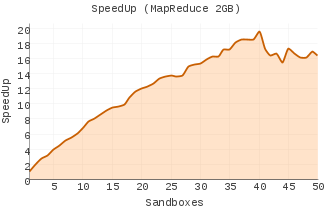
\includegraphics[scale=2.5]{SpeedUp_MapReduce_2GB_Small}
	\caption{SpeedUp MapReduce with 2GB.}
	\label{fig:SpeedUp_MapReduce}
\end{figure}


In figure~\ref{fig:SpeedUp_MapReduce} we can observe how the efficiency of the execution drops as the number of Sandboxes increases. As more execution points are added, the overhead of communication, disk I/O, and scheduling increases. We observe how the efficiency drops from 97\% with 2 Sandboxes, to 33\% with 50 Sandboxes.


%EFFICIENCY
\begin{figure}	
	\centering
	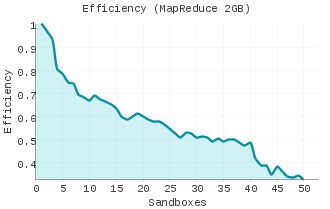
\includegraphics[scale=2.5]{Efficiency_MapReduce_2GB_small}
	\caption{Efficiency MapReduce with 2GB.}
	\label{fig:Efficiency}
\end{figure}

We observed significant speedUp and efficiency if we consider the fact that our system still in a prototypical stage and we haven’t implemented important optimizations and tuning. The Server, Client and Sandbox components of this experiment were remotely located, i.e. all communication was over the internet and not in a LAN.


\subsection{Overhead}

In the second experiment, we measured the task creation overhead of JSpeed.io in comparison with the Message Passing Interface (MPI). Using 18 Quad-Core machines, we incrementally deployed an empty task(no computation) in multiples of 18. As we can observe in figure 9, JSpeed outperforms MPI in the first 40 task deployments, then the overhead behaves almost linearly constant until approximately 90 tasks. MPI would scale pretty well horizontally while our system will reach a bottleneck in the communication after 90. Figure~\ref{fig:Overhead} shows how the JSpeed.io overhead drastically increases when the single-threaded server reaches the communication limit. In the next version of JSpeed.io, the Server will be scaled horizontally by using a load balancer~\cite{Nginx}, and multiple processes connected via a key-value cache and store~\cite{Redis}.

%OVERHEAD
\begin{figure}	
	\centering
	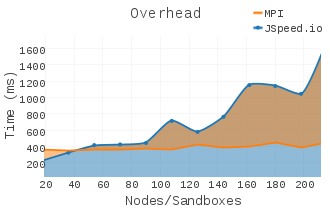
\includegraphics[scale=3.0]{Overhead}
	\caption{JSpeed.io and MPI task creation overhead.}
	\label{fig:Overhead}
\end{figure}


Our third experiment consists of approximating PI with the Monte Carlo method. Since our prototype’s Server component is currently single threaded, we executed the benchmark in 16 machines to keep the task creation overhead low. In figure 10 we can observe how JSpeed.io compares with MPI at different execution iterations(from 108 to 109).

%PI Approximation
\begin{figure}	
	\centering
	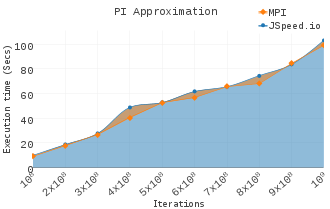
\includegraphics[scale=3.0]{PI_Approximation} %PI_Approximation
	\caption{JSpeed.io and MPI Monte Carlo PI approximation.}
	\label{fig:PI}
\end{figure}

The results shown in figure~\ref{fig:Overhead} raises a common question: How is an execution in Javascript almost as fast as native compiled C code? The answer is a combination of many factors. First, the native MPI execution is faster in the context of each node. On other hand, JSpeed.io has low task deployment overhead as we saw in figure 8. Another factor is that the V8 engine highly optimizes Javascript code via its Dynamic Machine Code Generation[28] that can lead to almost native performance.


\subsection{Scaling}
\begin{figure}[h]	
	\centering
	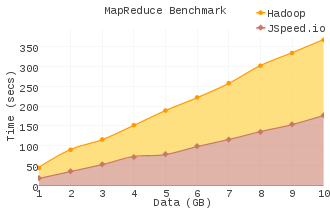
\includegraphics[scale=3.0]{MapReduce_Benchmark}
	\caption{JSpeed.io and Hadoop MapReduce Job Scaling from 1GB to 10GB datasets.}
	\label{fig:JobScaling}
\end{figure}

In our fourth experiment, we benchmark the scaling of Hadoop MapReduce and JSpeed.io’s. After measuring processing time of all datasets(1GB-10GB) on both systems, we observed a noticeable difference in the linear scaling.

As shown in figure~\ref{fig:JobScaling}, JSpeed.io linear execution times grows slower than those in Hadoop. Both systems ran on the same machines, with equivalent algorithms, and generate the same results. Figure~\ref{fig:JobScaling} shows the difference in completion times on both systems. The 10GB dataset took 367 and 176 seconds to complete with Hadoop and JSpeed.io respectively. With a difference of 197 seconds, JSpeed.io process the biggest dataset 2.09 times faster than Hadoop. These results, although hard to believe, have a simple explanation. Hadoop is way more complete and robust than our system, and can scale up to terabytes of data. JSpeed.io is currently limited to relatively small datasets and lacks basic features, such as execution checkpoints, group communication(the prototype), sophisticated fault tolerance, and many other elements that cause overhead in the overall execution flow but are completely necessary. Another JSpeed.io limitation is the  ~1.7GiB (64 bits) and ~1 GiB(32bits) of RAM consumption limit per Sandbox due to the V8 engine internals, although this may change in the near future.  JSpeed.io is designed as a general purpose distributed platform, and in this experiment we demonstrated the capabilities of emulating algorithms such as MapReduce.


\section{Future Work}

Although we have presented the potential of this system, you could say that is far from being a complete and robust system. We currently have a long roadmap of features and basic components that must be implemented. Important tasks in our roadmap include but is not limited to:

Structural changes: The system's structure still in its conceptual phase. We need to restructure all components to follow a robust distributed pattern. A major task is to fully integrate WebRTC~\cite{Vogt2013} for dynamic and transient connectivity between Sandboxes, i.e. the dynamic creation of topology overlays on each Job’s deployment.
Programming interface: Programming interface must be formalized. This includes the event-driven finite state machine model, single/group communication operations, third party libraries importing, and a clear guide of how to implement synchronization in every possible scenario.

Fault Tolerance: We need to implement two main fault tolerance approaches, one for batch jobs, and another for  streaming jobs. Both approaches must deal with the transient nature of our system. i.e. Sandboxes leaving and entering the system at any point of a computation. This is one of the most important and challenging tasks in our roadmap.
Optimization and porting: An important task in our future work is to take advantage of several optimization techniques for the deployed job’s code. From static code optimization and transformation to the possibility of porting any language that can compile to  LLVM into pure Javascript code~\cite{Zakai2011}. Our system needs to exploit all performance technologies and improvements in order to yield high performance at each distributed execution.

Security: Security and privacy are a concern. We need to do an exhaustive analysis of the different scenarios where our system could become harmful or a threat to the user’s privacy or system. We will be implementing state of the art and novel approaches to ensure the robustness and fidelity our system.

Additional to all tasks mentioned above, we plan to perform a wider and a detailed comparison between JSpeed.io and current leading systems/frameworks~\cite{Hadoop,GroppWilliamandLuskEwingandSkjellum1999}. We will cover important aspects such as power consumption, memory usage, network usage, and failure recovery under different workloads and scenarios.


\section{Related Research and Systems}
Our goals are analogous to those of volunteer computing projects such as CrowdCL~\cite{MacWilliam2013}, SETI@Home~\cite{Korpela2001a}, because they work on the premise that users can willingly contribute idle CPU cycles in order to solve large-scale computational problems.  In addition, JSpeed.io implements parallelism and sandboxing techniques using a JavaScript based framework similar to River Trail~\cite{Herhut2013a} and JSand~\cite{Agten2012}.

MacWilliam et al. achieved the simplified development of web-based GPU applications through a volunteer computing framework called CrowdCL~\cite{MacWilliam2013}. CrowdCL consists of client and server components that provide an open-source volunteer computing framework. CrowdCL’s client framework allows developers to run Javascript code in the background of web browsers. Developers can use the CrowdCL’s framework to write OpenCL applications using Javascript, distribute computations to the user's web browser clients, and finally gather results on the server[4]. On the other hand, our framework affords distributed execution of JavaScript implemented kernels using volunteer’s  web browsers. 

SETI@home~\cite{Korpela2001a} is a scientific experiment that uses Internet-connected computers in the search for extraterrestrial intelligence. The BOINC project provides the framework that powers SETI@home.  SETI@home has reached hundreds of TeraFlops from volunteer computing running on desktop applications. Their approach is to divide independent data from observations into small chunks that a personal computer can handle and analyze. In this way, they can distribute the work to people willing to donate their spare CPU cycles~\cite{Korpela2001a}. SETI@Home is a native desktop application, in contrast JSpeed.io is based on web technologies capable of executing on both user’s web browser and native Node.js runtime. 

River Trail provides deterministic parallelism to JavaScript applications. Moreover, River Trail is a parallel programming model and API for JavaScript which allows utilization of multiple cores, vector instructions, and GPUs on the user's web browser~\cite{Herhut2013a}. Similarly, JSpeed.io utilizes asynchronous parallelization techniques on the sandboxes improving performance. Our system is not an API, but a combination of emerging web technologies that form a distributed system running on top of the JavaScript runtime. In other words, technologies such as WebCL and River Trail can be easily integrated to improve JSpeed.io’s performance. 


\section{Conclusions}

We presented the JSpeed.io distributed system. With quick setup, maintainability, scalability, simple programming model, and performance, we aim to provide a powerful and straightforward platform to process distributed algorithms in a simpler manner. We presented examples of common algorithms and our vision of potential applications by exposing its benefits and drawbacks. The implemented programming model abstracted as a finite state machine aims to create high performance/non-blocking distributed algorithms without the need of any concurrent primitive such as locks, semaphores, and mutexes.We exposed the linear scaling or our system and how it can be used on different platforms such as web browsers and standalone ECMAScript runtime (Node.js). By easing the implementation, deployment, and maintainability of distributed algorithms, our contributions aims to attract scientists of all fields to immerse into big data processing and distributed computation.


\acks

We thank Purdue’s CS Department for providing the resources to test our system and generate the necessary results of our work. We also thank Agustin Bazzani for helping us to implement several algorithms for our system. Finally but not less important, we thank our friend Ruben O. Varela for helping with the orchestration deployment and setup of our system.

% We recommend abbrvnat bibliography style.

\bibliographystyle{abbrvnat}

% The bibliography should be embedded for final submission.

\bibliography{JSpeedIO}{}

%\begin{thebibliography}{}
%\softraggedright


%\end{thebibliography}


\end{document}